\documentclass[a0paper,portrait]{baposter}

\usepackage{wrapfig}
\usepackage{lmodern}

\usepackage[utf8]{inputenc} %unicode support
\usepackage[T1]{fontenc}
\usepackage{multicol} % Multi Columns
\usepackage{enumitem}

\usepackage{lipsum}
\usepackage{courier}
\usepackage{etex} 
\usepackage{graphics}
\usepackage{textcomp} 

\usepackage{xcolor}
\usepackage{colortbl}
\usepackage{tabu}

\usepackage{smartdiagram}
\usepackage{listings}

\selectcolormodel{cmyk}

\graphicspath{{figures/}} % Directory in which figures are stored


\newcommand{\compresslist}{%
\setlength{\itemsep}{0pt}%
\setlength{\parskip}{1pt}%
\setlength{\parsep}{0pt}%
}


\definecolor{myblue}{rgb}{0,0,0.70}
\definecolor{myred}{rgb}{0.8,0,0}
\definecolor{mydarkgreen}{rgb}{0,0.55,0}
\definecolor{fibeamer@blue}{HTML}{3333B3}


% Code listings
\lstset{%
  basicstyle=\footnotesize\ttfamily,
  breakatwhitespace=false,
  breaklines=true,
  commentstyle=\color{green!60!black},
  extendedchars=true,
  keywordstyle=\color{fibeamer@blue},
  showspaces=false,
  showstringspaces=false,
  showtabs=false,
  stringstyle=\color{violet}
}

\newenvironment{boenumerate}
  {\begin{enumerate}\renewcommand\labelenumi{\textbf\theenumi.}}
  {\end{enumerate}}

\begin{document}

\definecolor{darkgreen}{cmyk}{0.8,0,0.8,0.45}
\definecolor{lightgreen}{cmyk}{0.8,0,0.8,0.25}
\definecolor{uniblue}{RGB}{0,102,153}

\setlist[1]{itemsep=-3pt}

\begin{poster}
{
grid=false,
headerborder=open, % Adds a border around the header of content boxes
colspacing=1em, % Column spacing
bgColorOne=white, % Background color for the gradient on the left side of the poster
bgColorTwo=white, % Background color for the gradient on the right side of the poster
borderColor=uniblue, % Border color
headerColorOne=uniblue, % Background color for the header in the content boxes (left side)
headerColorTwo=uniblue, % Background color for the header in the content boxes (right side)
headerFontColor=white, % Text color for the header text in the content boxes
boxColorOne=white, % Background color of the content boxes
textborder=rounded, %rectangle, % Format of the border around content boxes, can be: none, bars, coils, triangles, rectangle, rounded, roundedsmall, roundedright or faded
eyecatcher=false, % Set to false for ignoring the left logo in the title and move the title left
headerheight=0.15\textheight, % Height of the header
headershape=roundedright, % Specify the rounded corner in the content box headers, can be: rectangle, small-rounded, roundedright, roundedleft or rounded
headershade=plain,
headerfont=\Large\textsf, % Large, bold and sans serif font in the headers of content boxes
%textfont={\setlength{\parindent}{1.5em}}, % Uncomment for paragraph indentation
linewidth=2pt % Width of the border lines around content boxes
}
{}
%
%----------------------------------------------------------------------------------------
%	TITLE AND AUTHOR NAME
%----------------------------------------------------------------------------------------
%
{
\textsf %Sans Serif
{Specifying binary file formats for TAIGA data sharing and reuse
}
} 
{\sf\vspace{0em}\\
$Elena~Korosteleva^{1,*}$, $Kryukov~A.^{1}$, $Bychkov~I.^{2,3}$, $Khmelnov~A.^{2,3}$, $Mikhailov~A.^{2}$, $Shigarov~A.^{1,2,3}$
\vspace{0.1em}\\
\small{1. Skobeltsyn Institute of Nuclear Physics, Lomonosov Moscow State University\\
2. Matrosov Institute for System Dynamics and Control Theory SB RAS\\
3. Irkutsk State University
\vspace{0.0em}\\
$^*$elkrs@yandex.ru}
}
{
\includegraphics[width=0.20\textwidth]{logo_var1.pdf}
}
 

\headerbox{1. Abstract}{name=introduction,column=0,row=0, span=3}{
The on-going project, Karlsruhe-Russian astroparticle data life cycle initiative, aims developing an open science system to be able to collect, store, and analyze astroparticle physics data having the TAIGA (http://taiga-experiment.info) and KASCADE (https://web.ikp.kit.edu/KASCADE) experiments as the examples. One of the important issues is how to archive raw binary data to support their availability and reusing in the future. This work demonstrates ways for specifying binary file formats for TAIGA data sharing and reuse. There are several binary file formats used currently in TAIGA project. They provide a representation of raw data obtained from TAIGA facilities, including HiSCORE, IACT, T133, and Grande. The long-term preservation of raw binary data as originally generated is essential for rerunning analysis and reproducing research results in future. In this case, the raw data should be well documented and accompanied by some readers (i.e. software for parsing these data). The neglect of the issues may lead to the need for a reverse engineering of their file binary formats in future. The goal of the work is to provide human readable formal format description, as well as tools for serialization/deserialization and validation of the raw data. Some of the state-of-the art tools for formal describing binary data formats can provide a good enough solution for the issues of raw astroparticle physics data documenting and parsing. The work considers two of them, KAITAI STRUCT (http://kaitai.io) and FLEXT (http://hmelnov.icc.ru/FlexT). Both allow to express a formal specification of a binary data format in their domain-specific languages and to generate program code for parsing files of the format. The work presents our experience of using these tools for formal describing TAIGA binary data formats, documenting, and parsing library generation. This study can be interested in other experiments where raw binary data formats remain weakly documented or some parsing libraries for contemporary programming languages are required. This work has been financial supported by RSF (grant No~18-41-06003).
}

\headerbox{2. Motivation}{name=motivation,column=0,below=introduction,span=1}{
  \vspace{0.1cm}
	\smartdiagramset{
		font=\tiny,
		module minimum width=1cm,
		module minimum height=0.5cm,
		text width=1.6cm,
		circular distance=2.2cm,
	}
\begin{center}
	\smartdiagram[circular diagram:clockwise]{Data Capture \linebreak \& Storage,
		Data Availability, Simulations \linebreak \& Methods, Analysis, Open Access \linebreak \& Education, Archive
	}
\end{center}
	\begin{center}
	  \tiny{Astroparticle Data Lifecycle}
	\end{center}

 \textbf{TAIGA formats:}
	 \begin{itemize}
	  	\item TAIGA-IACT
	  	\item TUNKA-HISCORE
  		\item TUNKA-133
  		\item TUNKA-REX  
		  \item TUNKA-GRANDE
	  \end{itemize}
    \textbf{Issue:}
	  \begin{itemize}
  		\item No documentation, no open raw data access API
  		\item How to verify and reuse raw data?  
  	\end{itemize}
		\vspace{0.17cm}
}

\headerbox{3. Solution}{name=solution,span=2,column=1,below=introduction}{ % To reduce this block to 1 column width, remove 'span=2'

\vspace{0.1cm}

	\begin{center}
		\smartdiagram[sequence diagram]{\small{Binary data}, \small{Specification}, \small{Parse library}}
  \end{center}

\vspace{0.1cm}

}

\headerbox{4. Kaitai Struct}{name=kaitai,span=2,column=1,below=solution}{ % To reduce this block to 1 column width, remove 'span=2'

  \begin{multicols}{2}
    \begin{minipage}{0.50\textwidth}
      \begin{flushleft}
        \textbf{Declarative:} describe the very structure of the data, not how you read or write it
			\end{flushleft}   

			\begin{flushleft}
        \textbf{Packed with tools and samples:} includes a \textit{compiler}, an \textit{IDE}, a \textit{visualizer} and library of format specs			
      \end{flushleft}   
			
			\begin{flushleft}
        \textbf{Free \& open source:} licensed under the following terms: GPLv3+~(Compiler and visualizer), MIT or  Apache~v2~(Runtime libraries)
      \end{flushleft}   
    \end{minipage}

    \begin{minipage}{0.40\textwidth}
      \begin{flushleft}
        \textbf{Language-neutral:} write once, use in all supported languages:	
				
				% sub columns
				\begin{multicols}{2}
				  \begin{minipage}{0.5\textwidth}
						\begin{itemize}
							\item C++/STL
							\item C\#
							\item Go (*)
							\item Java
							\item JavaScript
						\end{itemize}
				  \end{minipage}
					
				  \begin{minipage}{0.5\textwidth}
						\begin{itemize}
							\item Lua
							\item Perl
							\item PHP
							\item Python
							\item Ruby
						\end{itemize}
				  \end{minipage}
        \end{multicols}
				%\vspace{0.1cm}
				%\scriptsize{(*) entry-level support}
				%\vspace{0.1cm}
      \end{flushleft}      
    \end{minipage}
  \end{multicols}
\vspace{0.1cm}
%Mikhail Yakshin, "`Kaitai Struct -- a new way to develop parsers for binary structures."', 2018. [Online]. Available: \url{https://kaitai.io}. [Accessed: 29- May- 2018]
}

\headerbox{5. HiSCORE specification diagram}{name=example,column=1, span=2, below=kaitai}{
	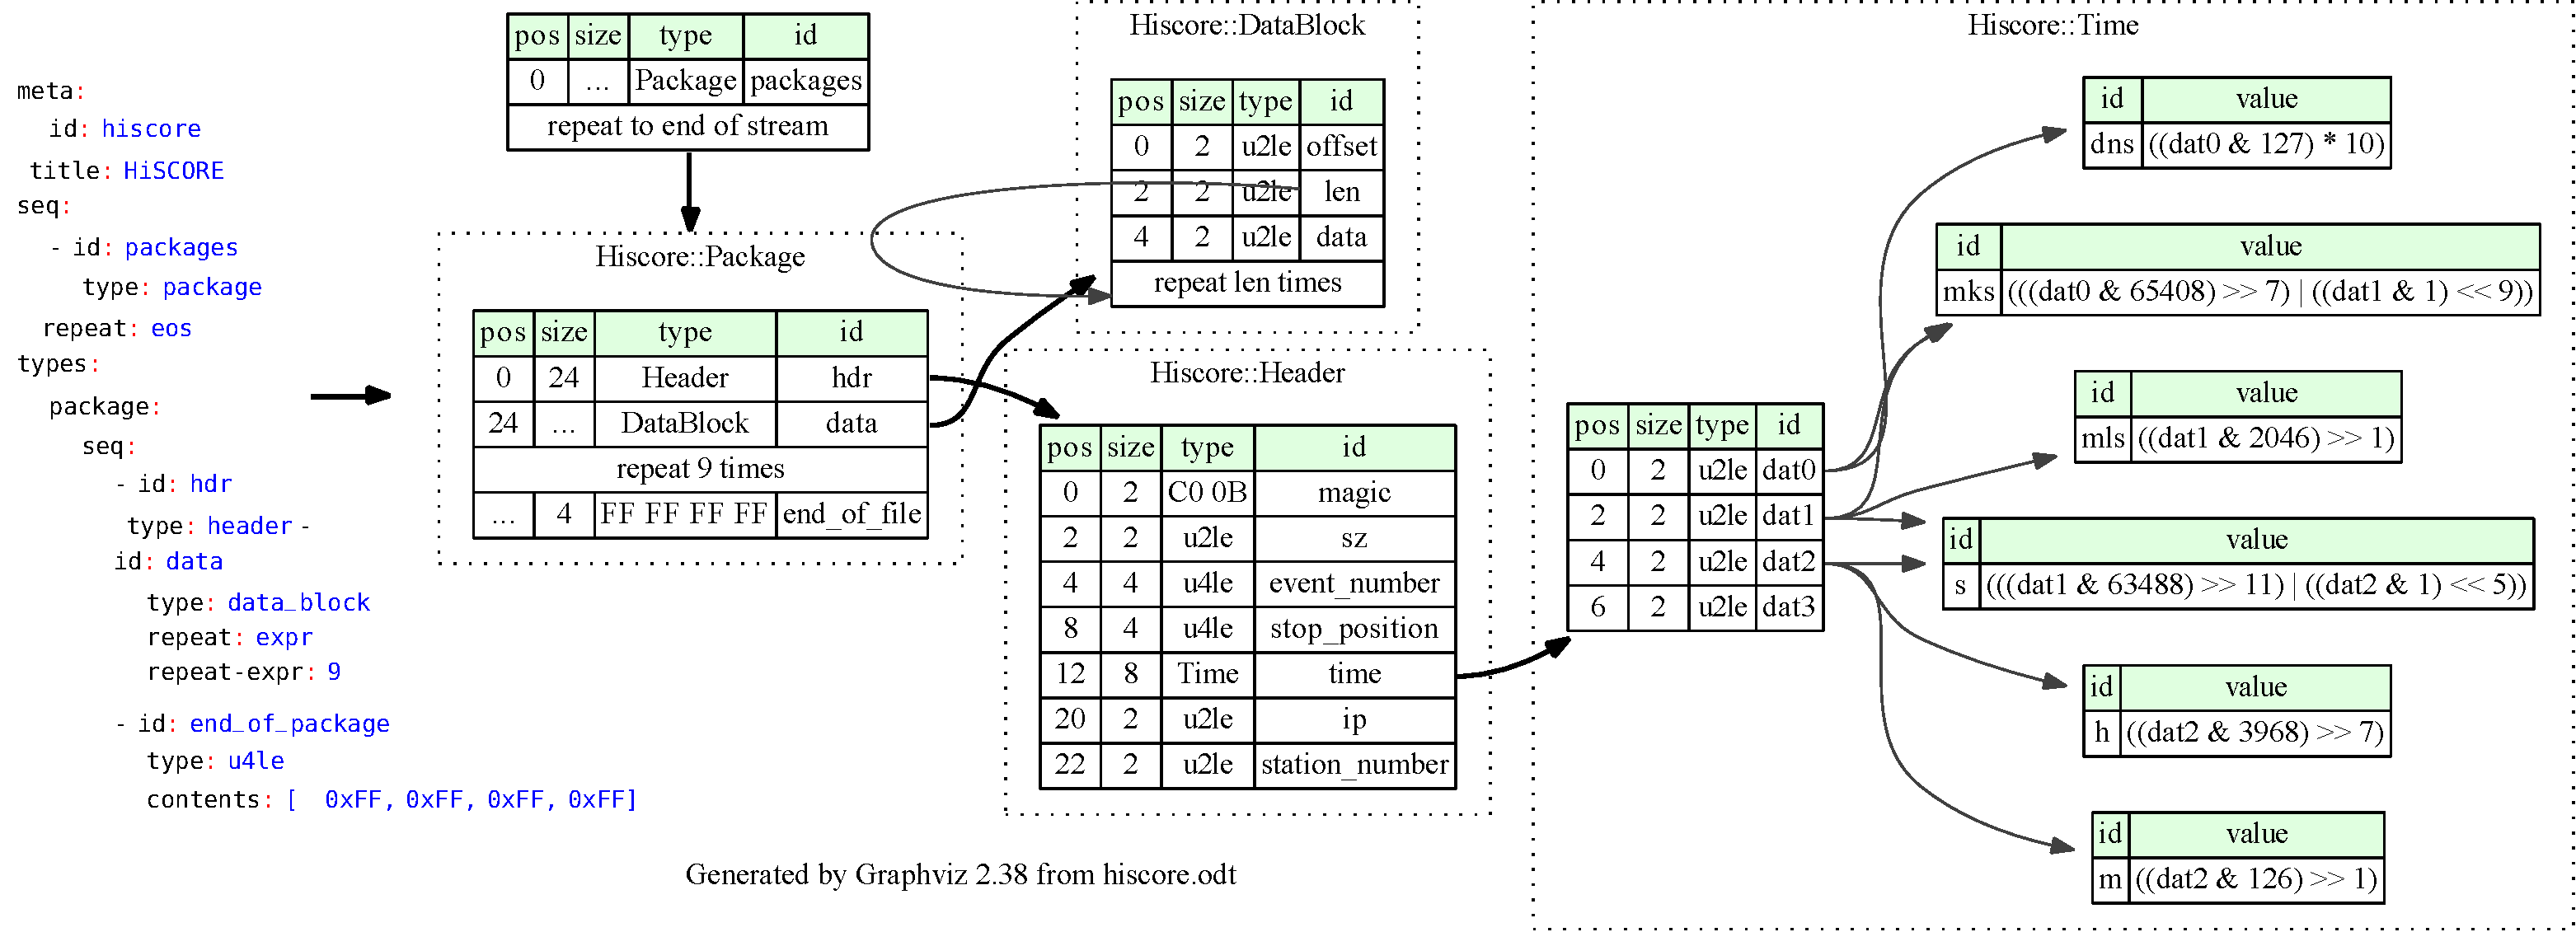
\includegraphics[width=1\textwidth]{hiscore.pdf}
}

\headerbox{6. How to use. C++ example}{name=src,span=1,column=0,below=motivation}{ % To reduce this block to 1 column width, remove 'span=2'
	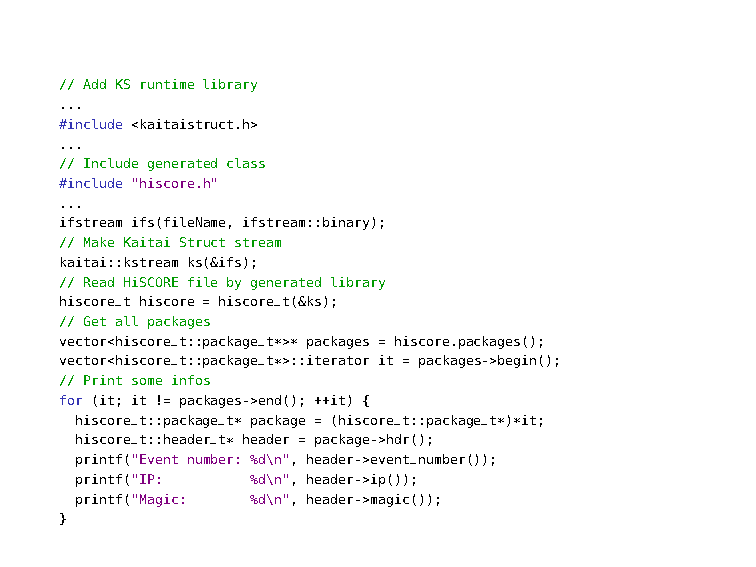
\includegraphics[width=1\textwidth]{src.pdf}
}

\headerbox{7. Results}{name=done,span=2,column=1,below=example}{ % To reduce this block to 1 column width, remove 'span=2'
	\begin{multicols}{2}
	  \begin{minipage}{0.45\textwidth}
			\vspace{0.1cm}
			\begin{itemize}
				\item TAIGA format specifications
				\item Reading libraries
				\item Examples for C++, Java, and Python 
				\item The libraries tested on real data
			\end{itemize}
		\end{minipage}
		\begin{minipage}{0.45\textwidth}
  		\vspace{0.1cm}
			\begin{itemize}
	  		\item GRANDE, T133, and TREX tested on $\approx$~89~000~files
				\item	HiSCORE, IACT tested on $\approx$~120~000~files  
			\end{itemize}
 			\begin{itemize}
	 			\item 4~\% of GRANDE, T133, and TREX files have BAD file format
				\item	0,6~\% of HiSCORE and IACT files have BAD file format		
			\end{itemize}
			\vspace{0.1cm}
		\end{minipage}	
	\end{multicols}		
}

\end{poster}
\end{document}
